\documentclass[xcolor=dvipsnames]{beamer} % dvipsnames gives more built-in colors
\mode<presentation>

\usetheme{Boadilla}

\definecolor{GWdarkblue}{HTML}{033C5A}

\usecolortheme[named=GWdarkblue]{structure}

% Sets the font
\usepackage[defaultfam,tabular,lining]{montserrat}
\setbeamerfont{title}{shape=\scshape}
\setbeamerfont{frametitle}{shape=\scshape}
%Remove "Figure" from captions
\setbeamertemplate{caption}{\raggedright\insertcaption\par}

\usepackage{graphicx}
\usepackage{tabularx}
\usepackage{hyperref}

\title[Predictive Election Models]{Predictive Election Models}
\author[SMPA 2152]{Data Analysis for Journalism and Political Communication (Fall 2024)}
\date{Prof. Bell}

\begin{document}

%%%%%%%%%%%%%%%%%%%%%%%%%%%%%%%%%%%%%%%%%%%%%%%%%%%%%%%%%%%%%%%%%%
\frame{
\titlepage
}

%%%%%%%%%%%%%%%%%%%%%%%%%%%%%%%%%%%%%%%%%%%%%%%%%%%%%%%%%%%%%%%%%%
\frame{\frametitle{Dart-Throwing Chimpanzees}

\centering
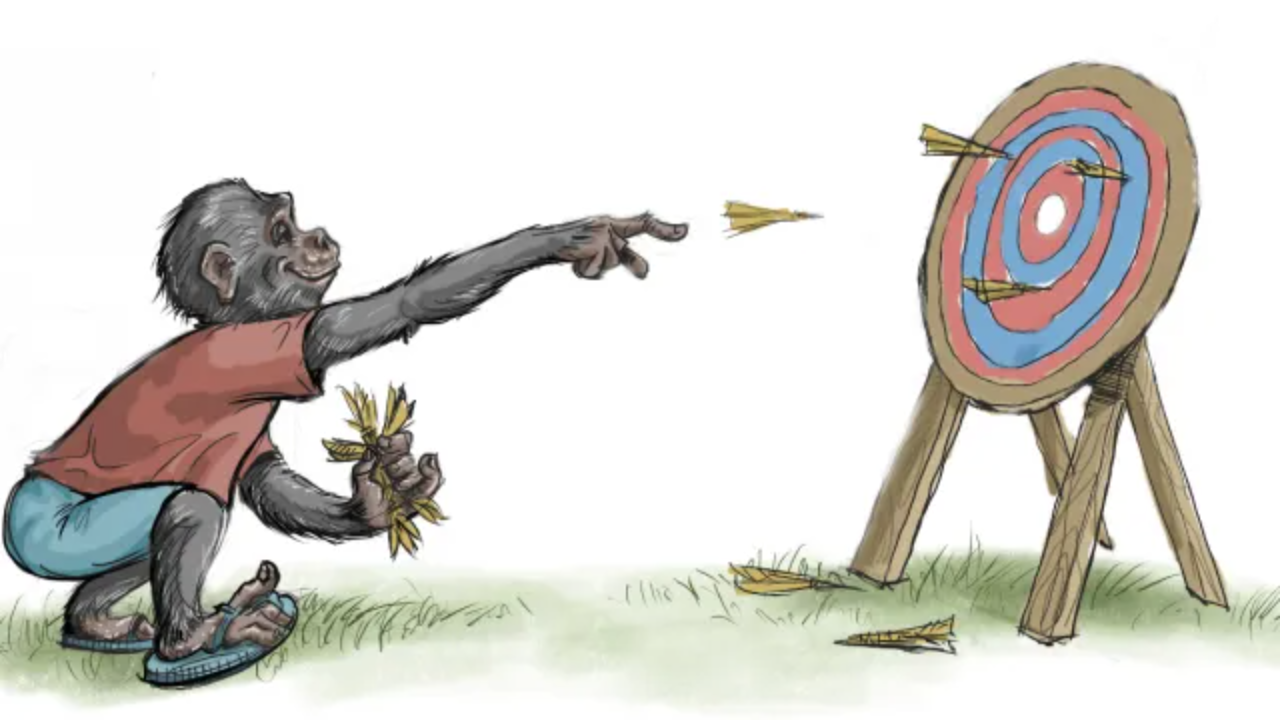
\includegraphics[width = .8\textwidth]{dart_throwing_chimps.png}
}

%%%%%%%%%%%%%%%%%%%%%%%%%%%%%%%%%%%%%%%%%%%%%%%%%%%%%%%%%%%%%%%%%%
\frame{\frametitle{Prediction}

\begin{itemize}[<+->]
    \item Prediction is not the same thing as inference
    \item Prediction uses \textbf{training data} to make predictions on \textbf{test data}
    \begin{itemize}
        \item With inference, we are generating an estimate from a sample that is representative of the population
        \item Prediction focuses on an ``out-of-sample'' population
    \end{itemize}
    \item Biggest risk in prediction is \textbf{overfitting}: generating a model that relies too heavily on the training data and is not able to make good predictions on the test data
    \begin{itemize}
        \item With inference, the larger the sample, the better
    \end{itemize}
    \item By design, the \textbf{prediction interval} is wider than the confidence interval (e.g., MOE)
\end{itemize}
}

%%%%%%%%%%%%%%%%%%%%%%%%%%%%%%%%%%%%%%%%%%%%%%%%%%%%%%%%%%%%%%%%%%
\frame{\frametitle{Machine Learning and AI}

\begin{itemize}[<+->]
    \item Machine learning is a wide spectrum ranging from simple decision trees to large language models
    \item The ``learning'' is simply that the data draws on patterns in the training data to make predictions on the test data
    \item It is ``machine'' learning because computation takes over some of the decisions that are usually left to the researcher
    \begin{itemize}
        \item \textbf{Supervised learning}: The researcher provides the machine with a target (e.g., an election outcome) and the machine determines the features of the test data that best predict the target
        \item<.-> \textbf{Unsupervised learning}: What we typically think of as ``artificial intelligence,'' the machine is not given a target and uncovers new patterns in the data
    \end{itemize}
    \item Because computation replaces some researcher decisions, many machine learning/AI models are considered ``black boxes'' where it is difficult to decipher why the machine makes the predictions that it does (called \textbf{explainability})
\end{itemize}
}

%%%%%%%%%%%%%%%%%%%%%%%%%%%%%%%%%%%%%%%%%%%%%%%%%%%%%%%%%%%%%%%%%%
\frame{\frametitle{Expert Political Judgment}

\centering
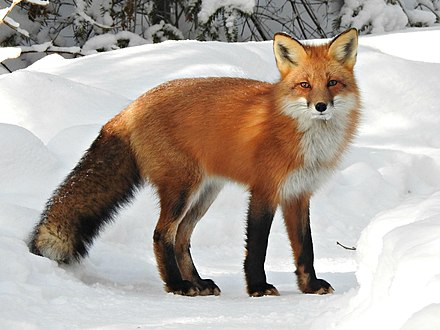
\includegraphics[width = .4\textwidth]{fox.jpg}
\hspace{2pt} vs. \hspace{2pt}
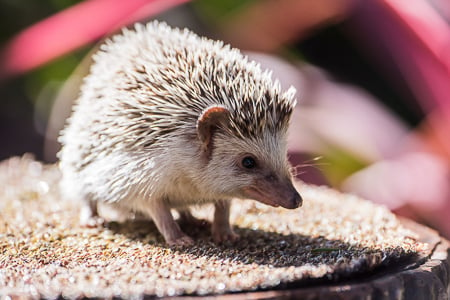
\includegraphics[width = .45\textwidth]{hedgehog.jpg}
}

%%%%%%%%%%%%%%%%%%%%%%%%%%%%%%%%%%%%%%%%%%%%%%%%%%%%%%%%%%%%%%%%%%
\frame{\frametitle{Wisdom of the Crowds}

\only<1>{
    \centering
    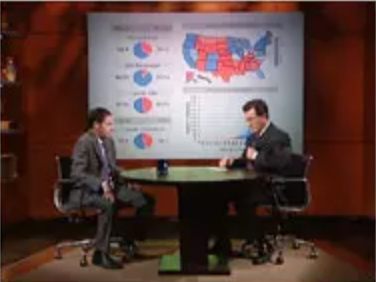
\includegraphics[height = .5\textheight]{silver_colbert.png}
}

\only<2>{
    \centering
    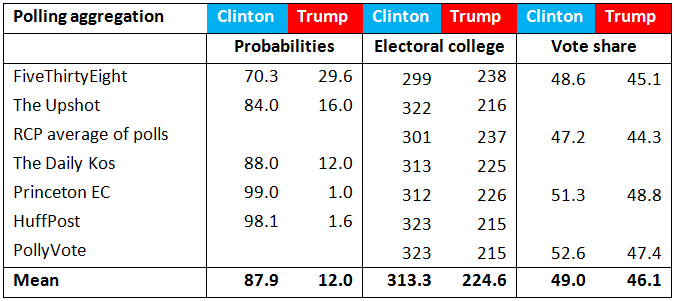
\includegraphics[width = .9\textwidth]{2016_predictions.png}
}

\only<3>{
    \centering
    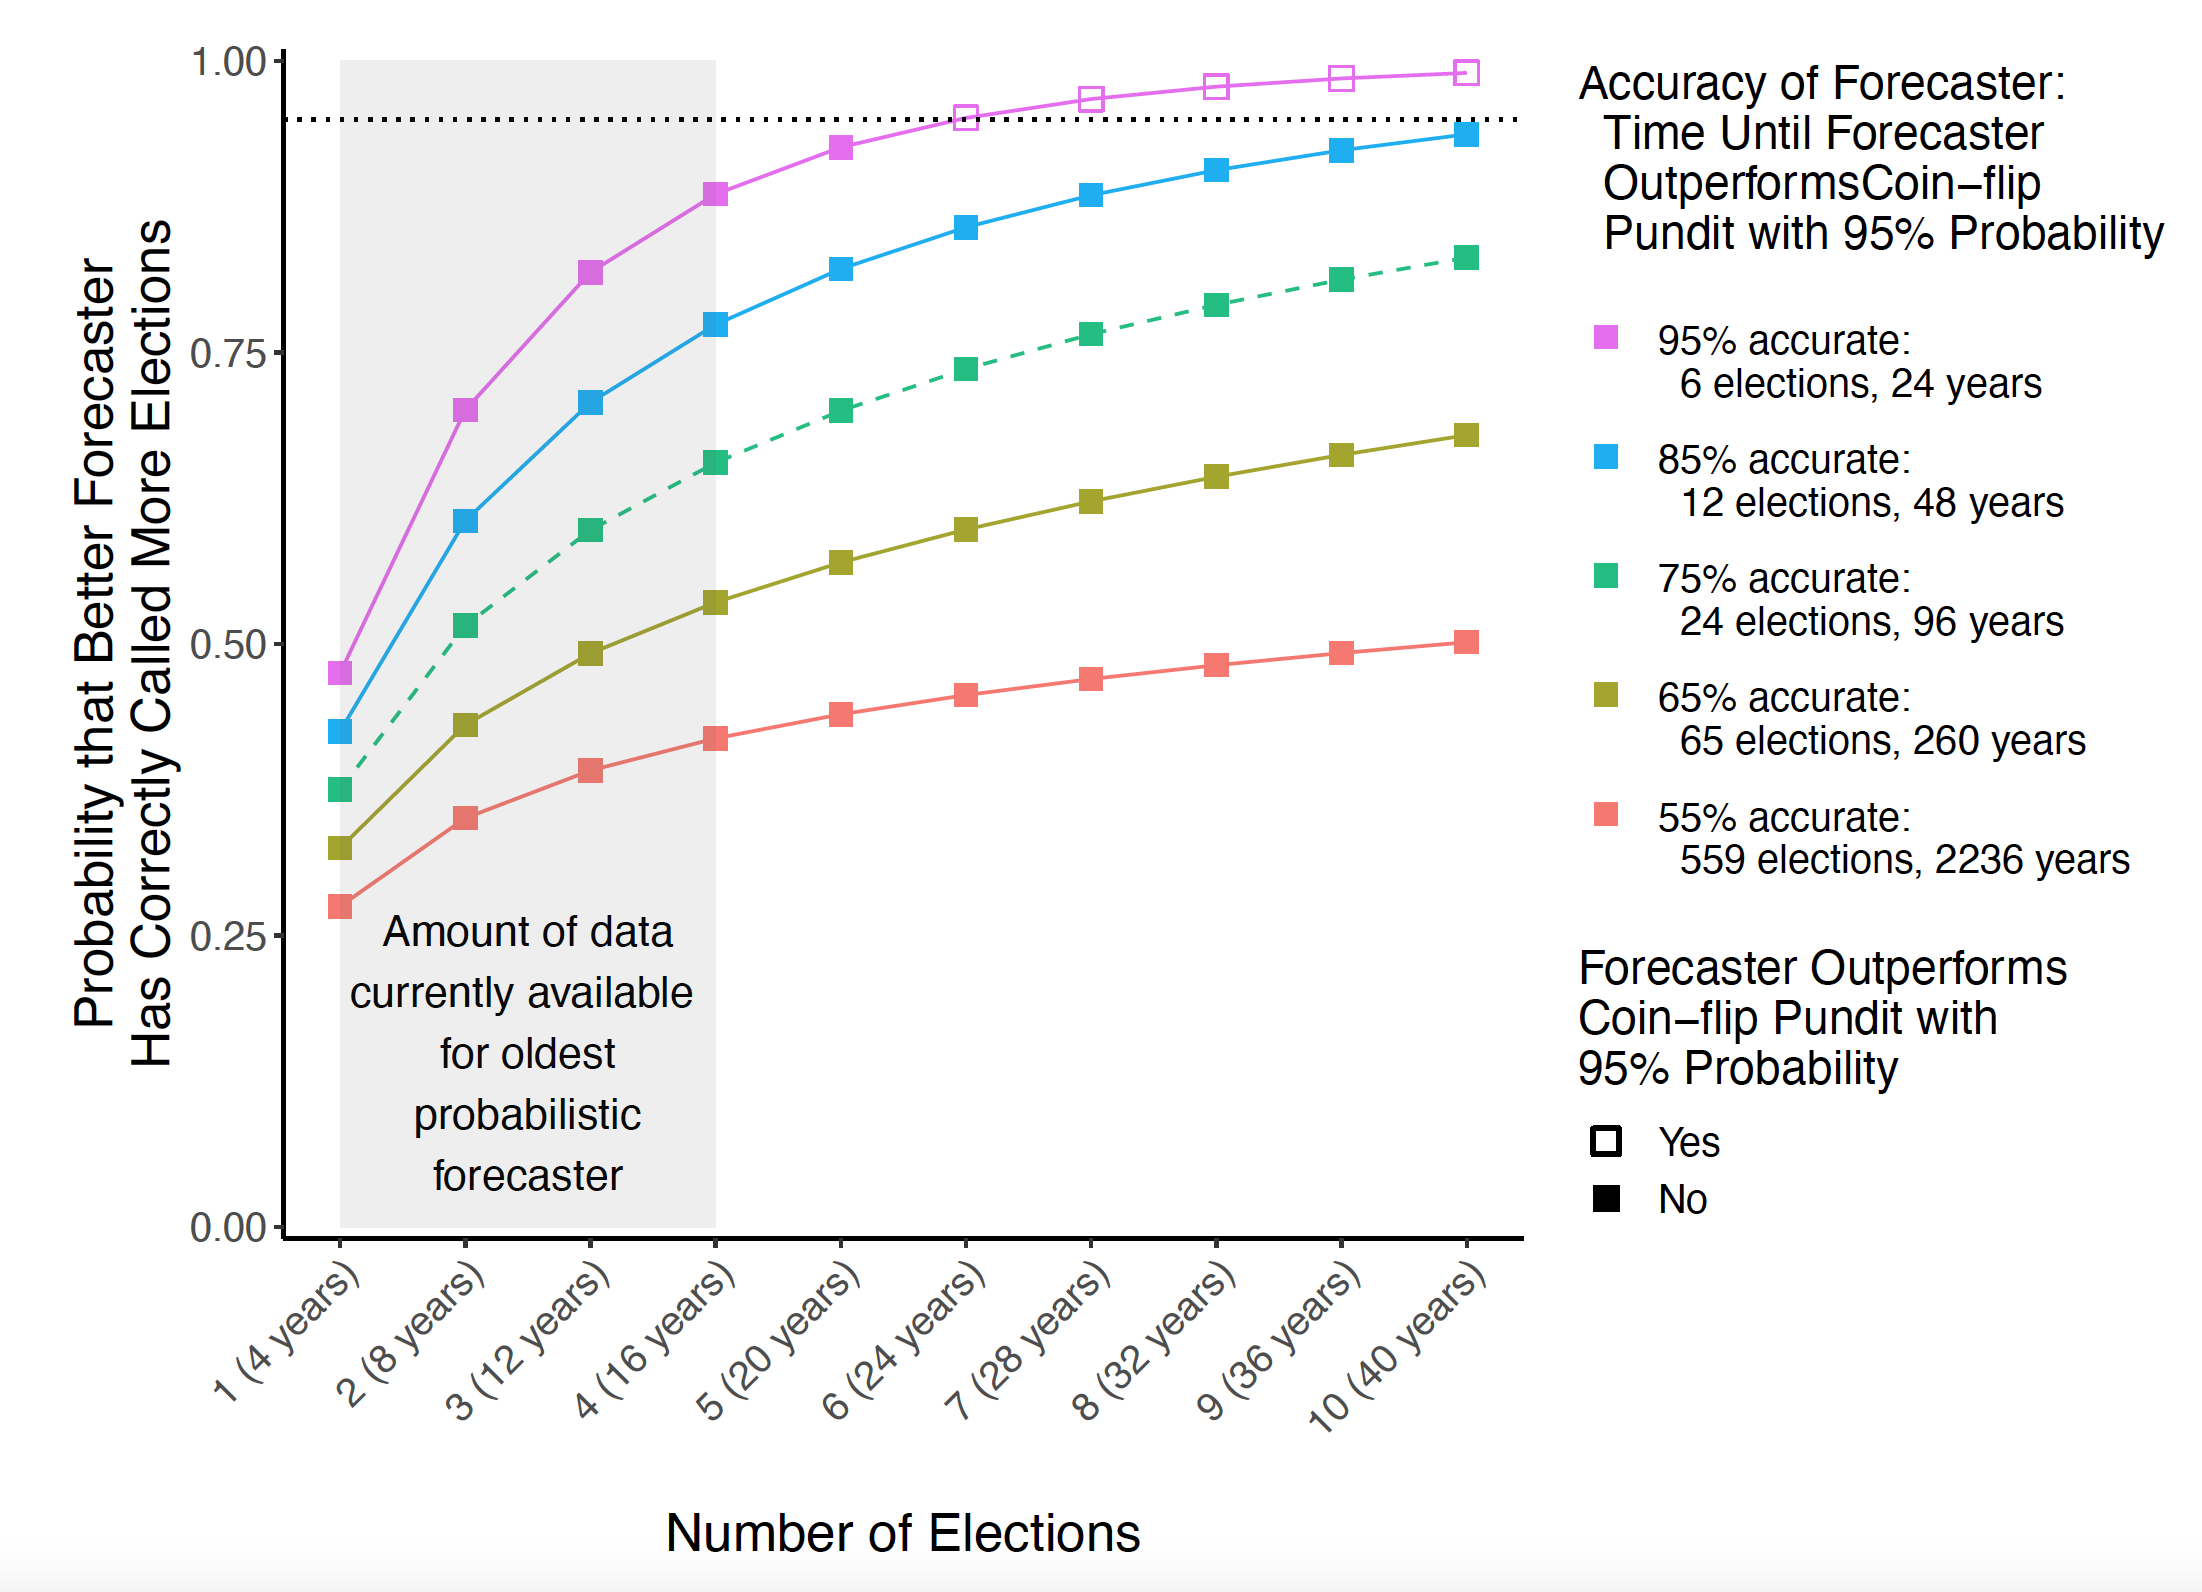
\includegraphics[width = .8\textwidth]{forecasting_accuracy.png} \\
    \tiny Source: Grimmer, Justin, Dean Knox, and Sean Westwood. 2024. ``Assessing the Reliability of Probabilistic US Presidential Election Forecasts May Take Decades.'' OSF Preprints. August 26. doi:10.31219/osf.io/6g5zq.
}
}

%%%%%%%%%%%%%%%%%%%%%%%%%%%%%%%%%%%%%%%%%%%%%%%%%%%%%%%%%%%%%%%%%%
\frame{\frametitle{How Prediction Models Work}

\only<1>{
    \centering
    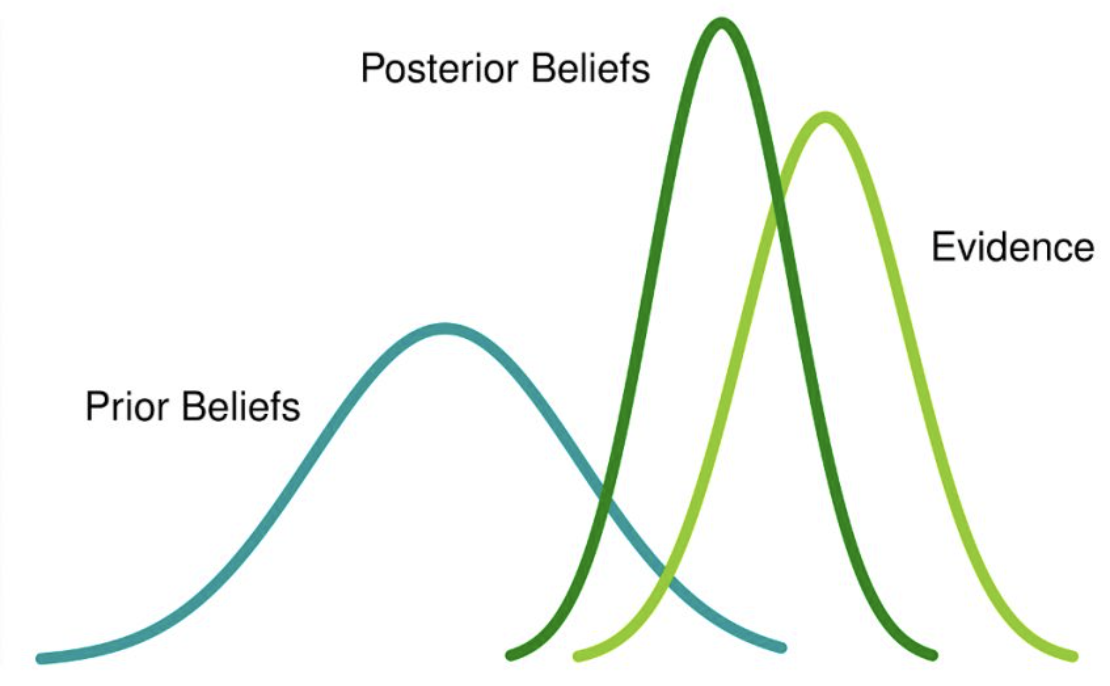
\includegraphics[width = .8\textwidth]{bayesian.png}
}

\only<2>{
    \centering
    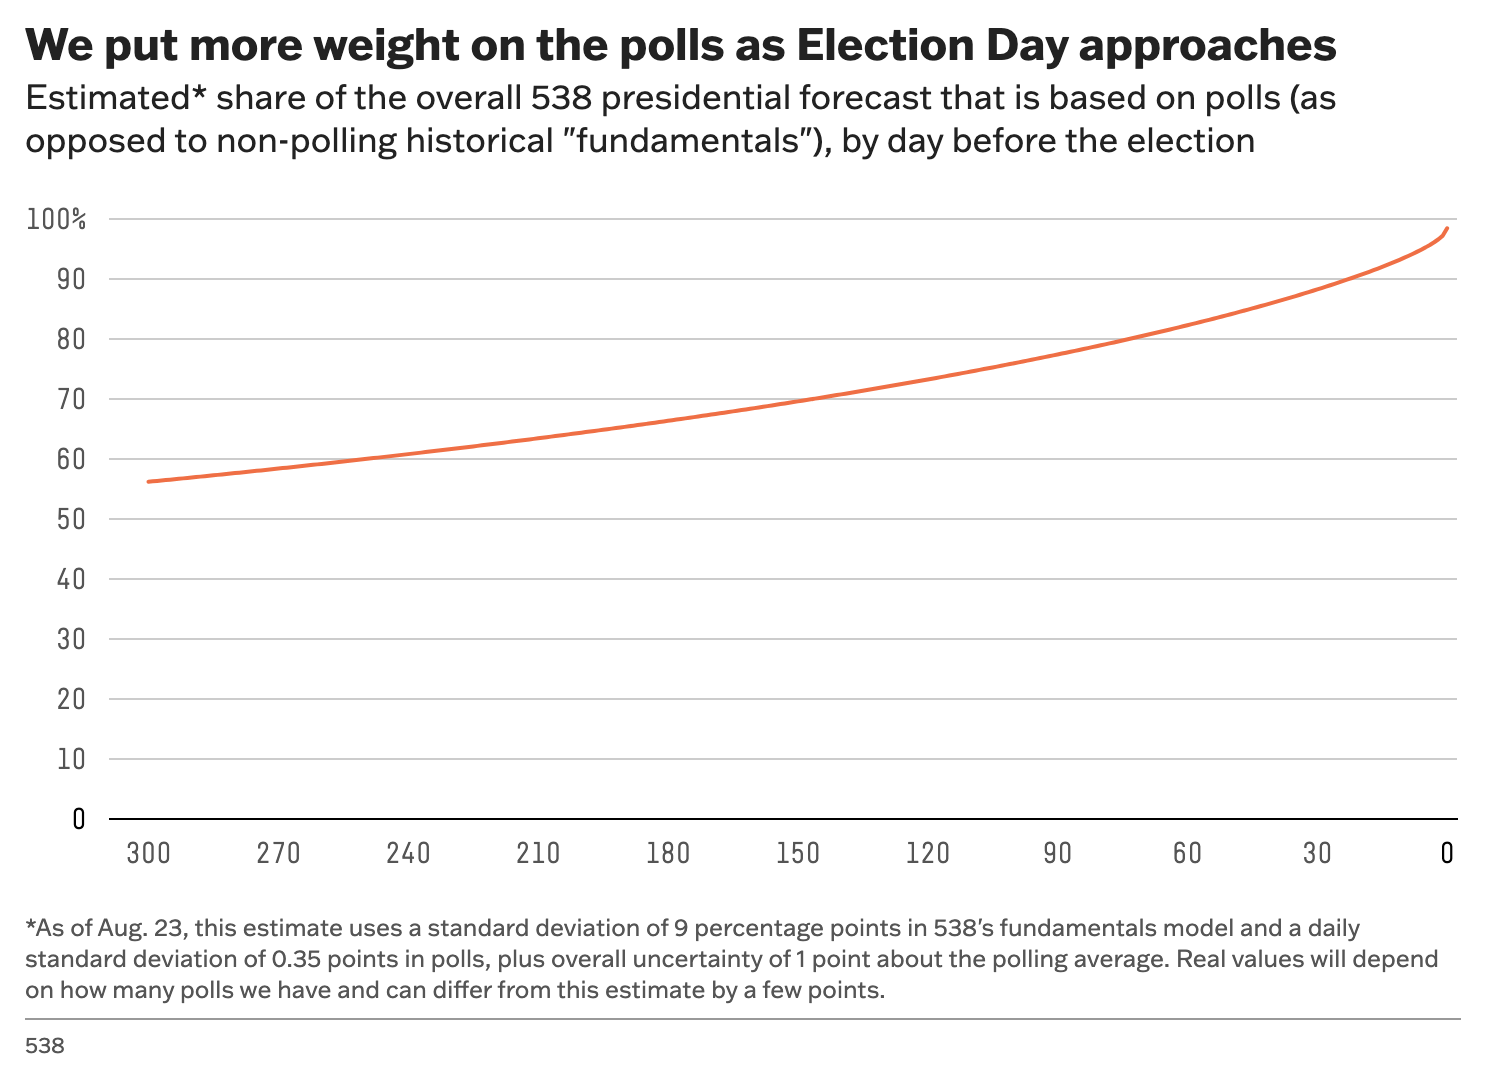
\includegraphics[width = .8\textwidth]{fundamentals_decay.png}
}

\only<3-5, 7-8>{
Election prediction models must decide:
    \begin{itemize}[<+(2)->]
        \item What polls to include (and how much to weight them): quality, quantity, sample size, time, etc.
        \item How to adjust polls for house effects and/or mode effects
        \item How to quantify the uncertainty in poll results
        \item<7-> How to model election outcomes (e.g, intra-state correlation)
        \item<8-> How to communicate probabilities
    \end{itemize}
}

\only<6>{
    \centering
    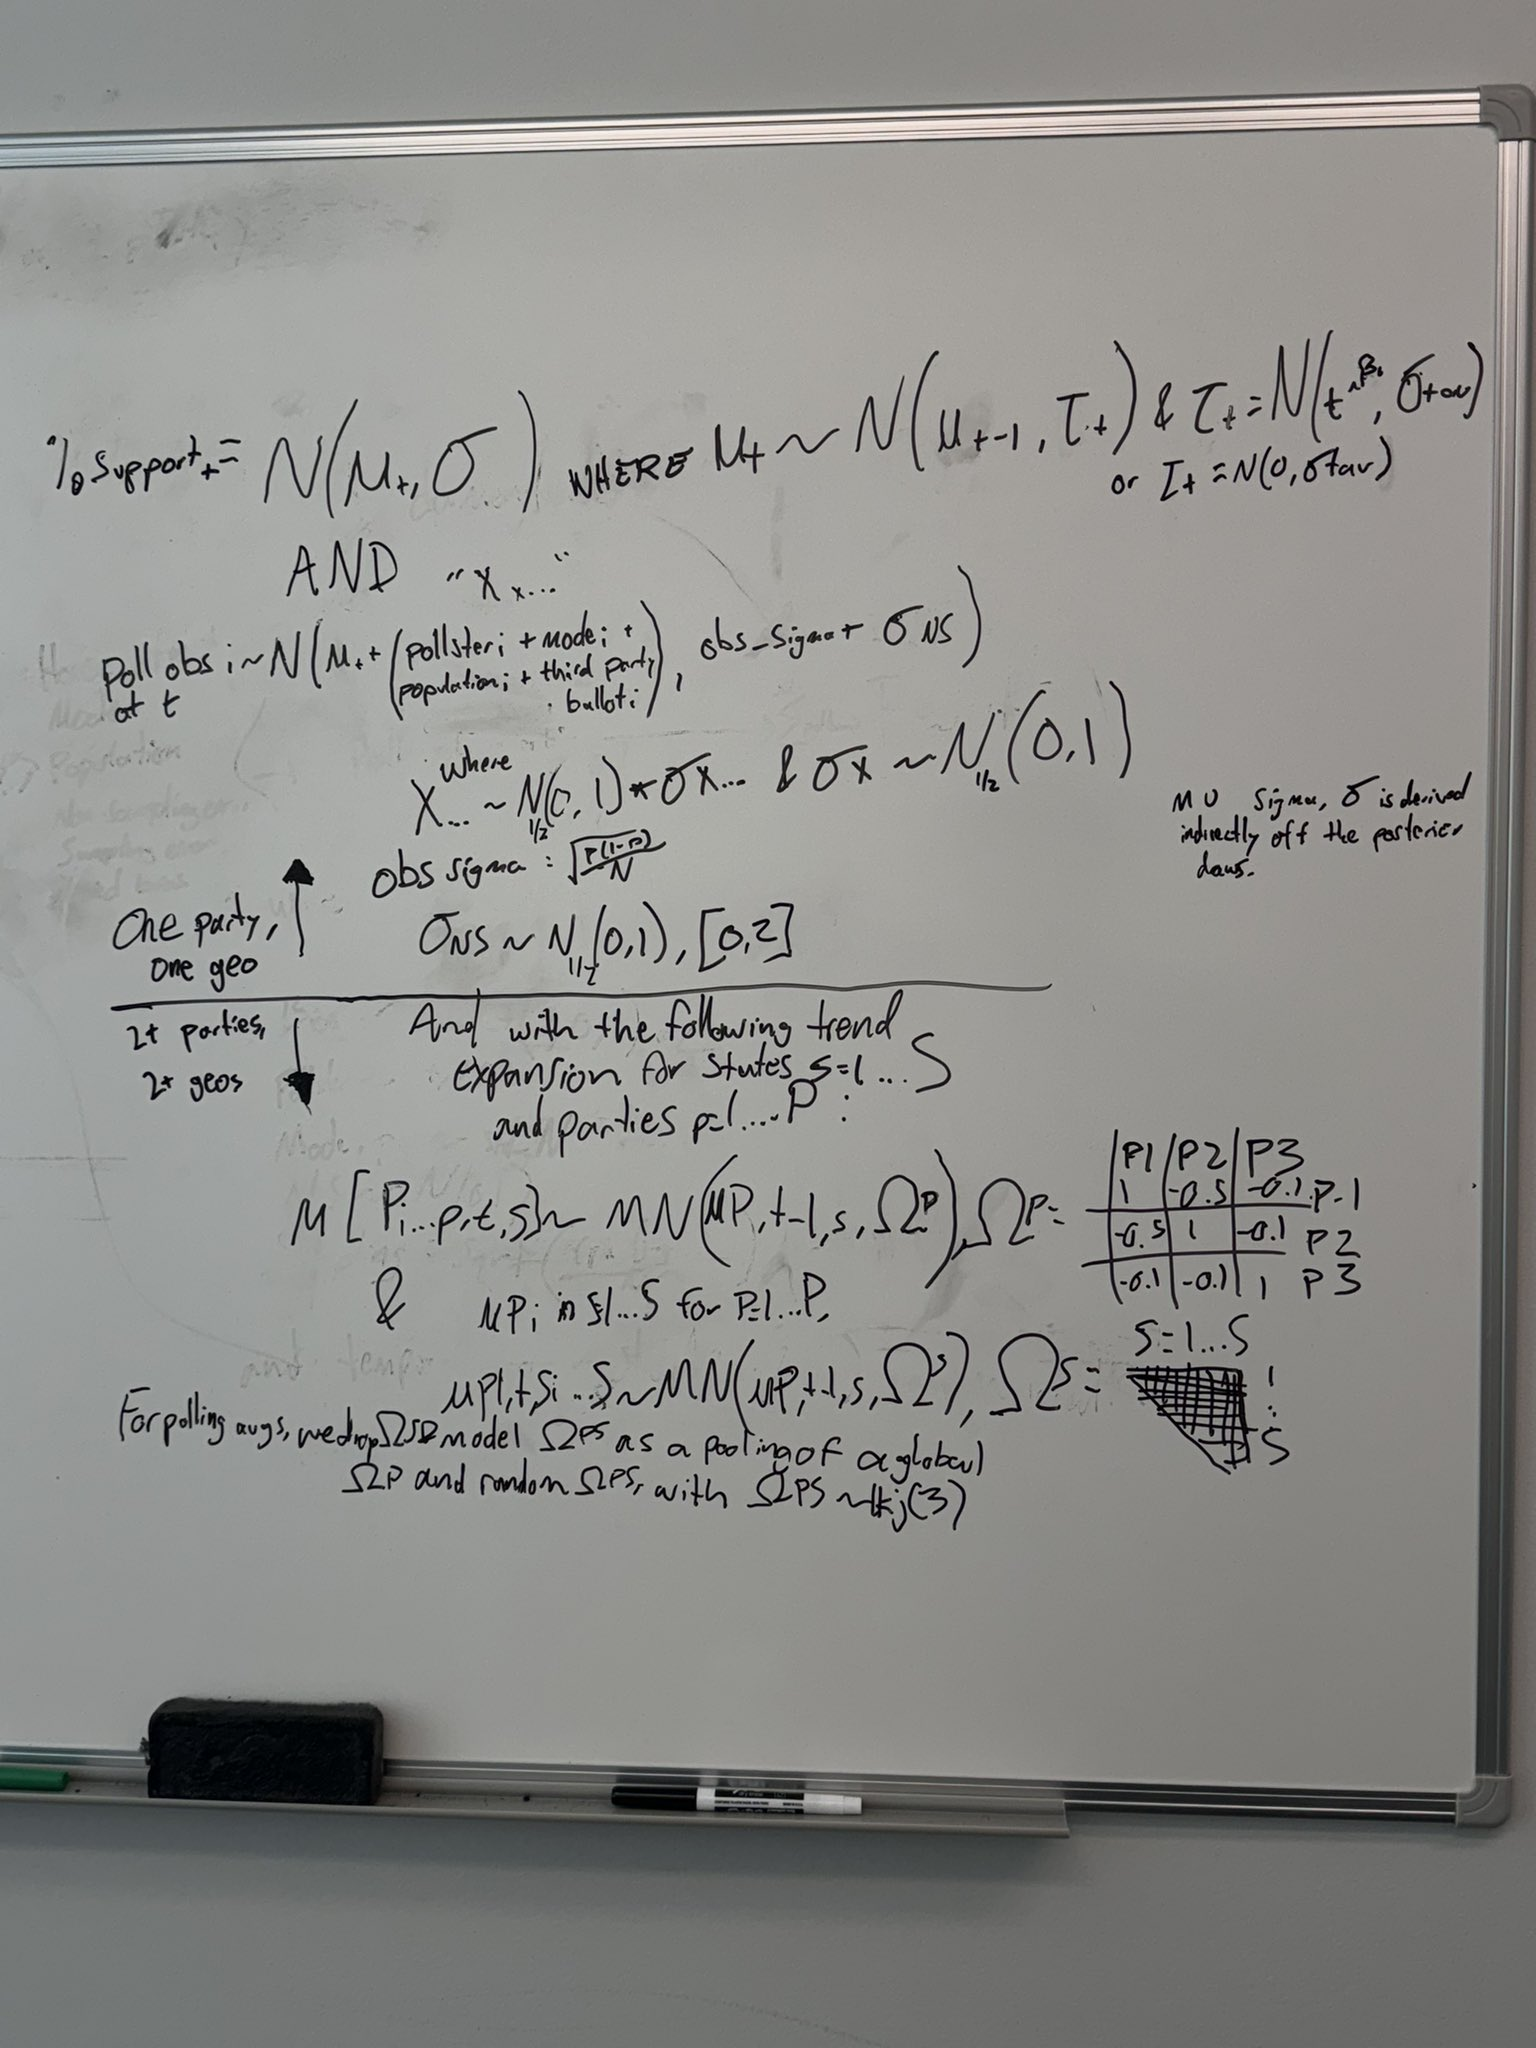
\includegraphics[height = .8\textheight]{morris_economist_whiteboard.jpeg}
}

\only<9>{
    \centering
    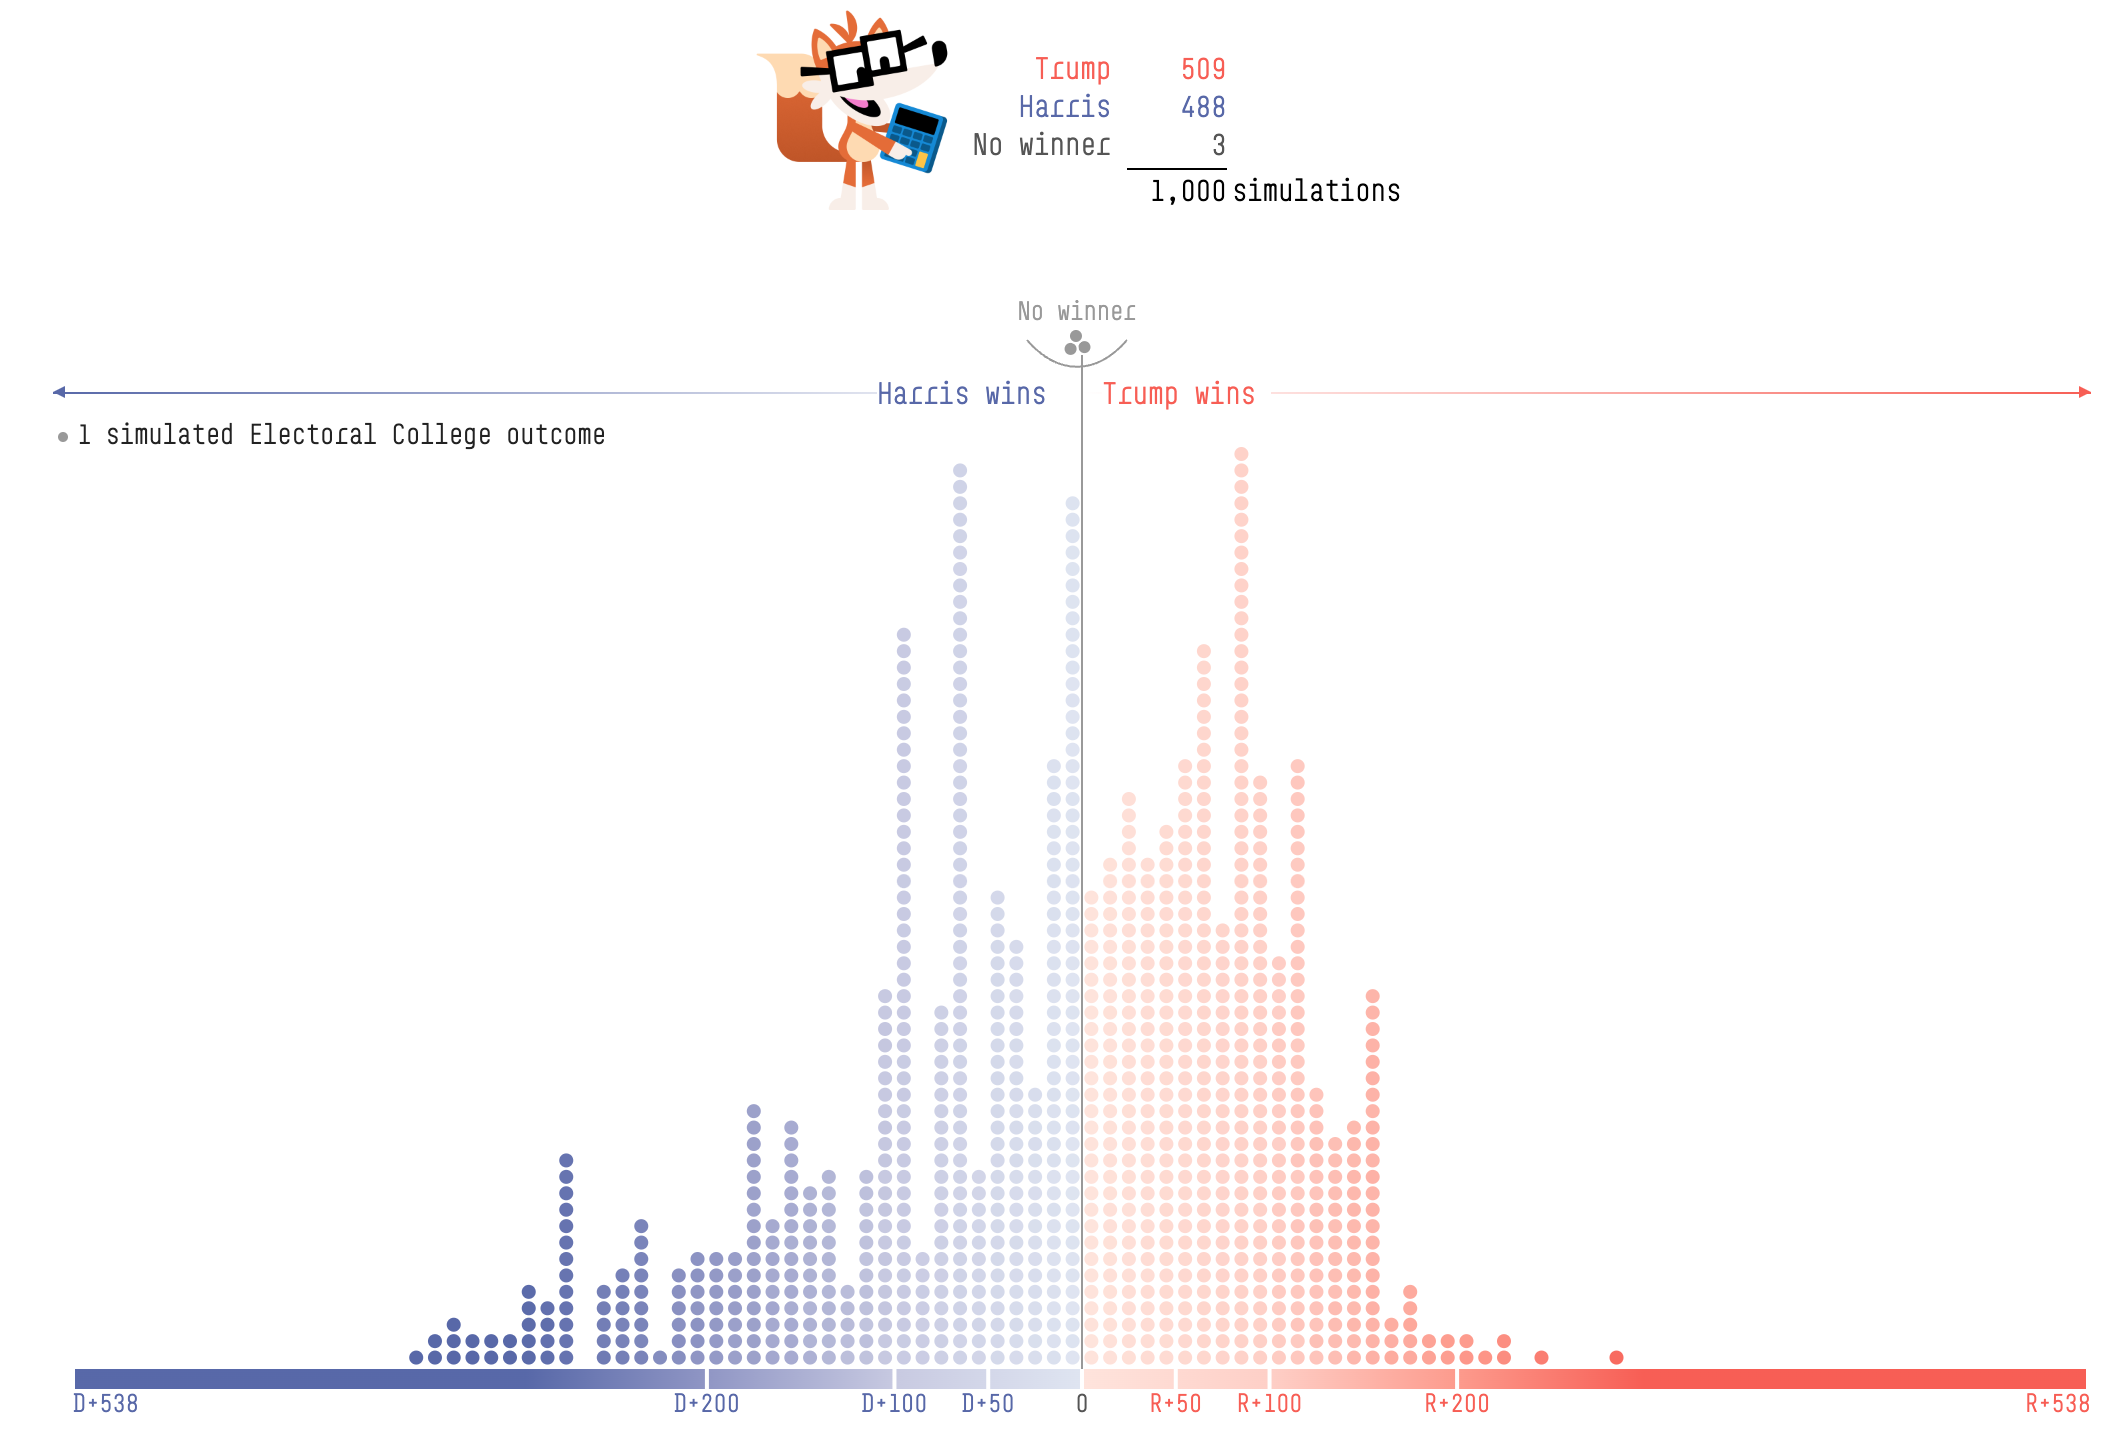
\includegraphics[height = .8\textheight]{fivethirtyeight_30oct.png}
}

\only<10>{
    \centering
    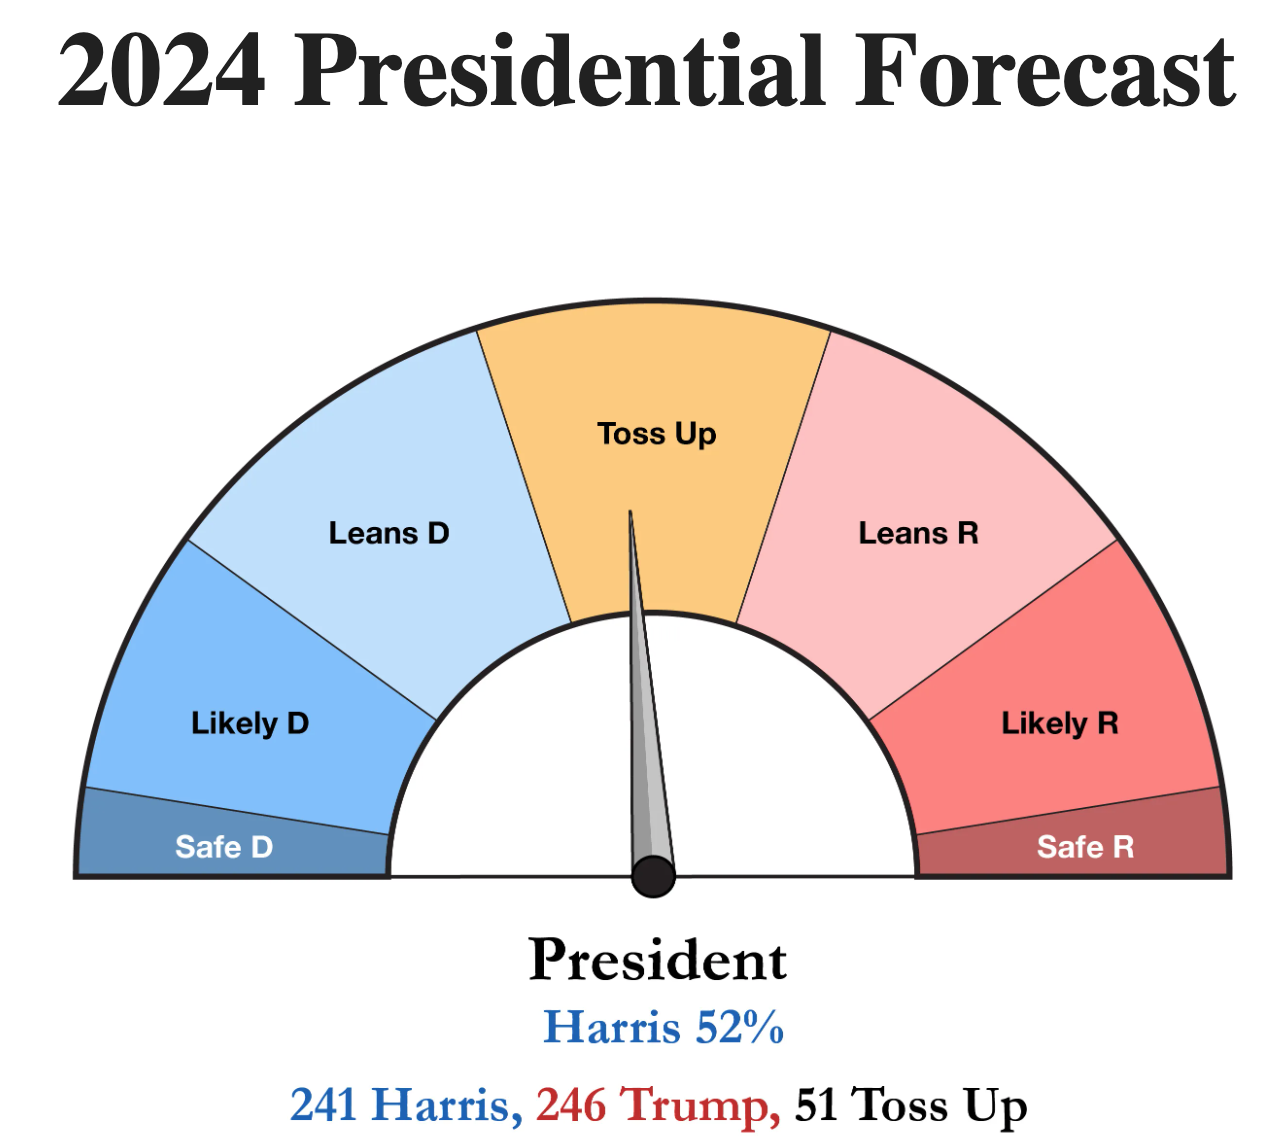
\includegraphics[height = .8\textheight]{split_ticket_30oct.png}
}

\only<11>{
    \centering
    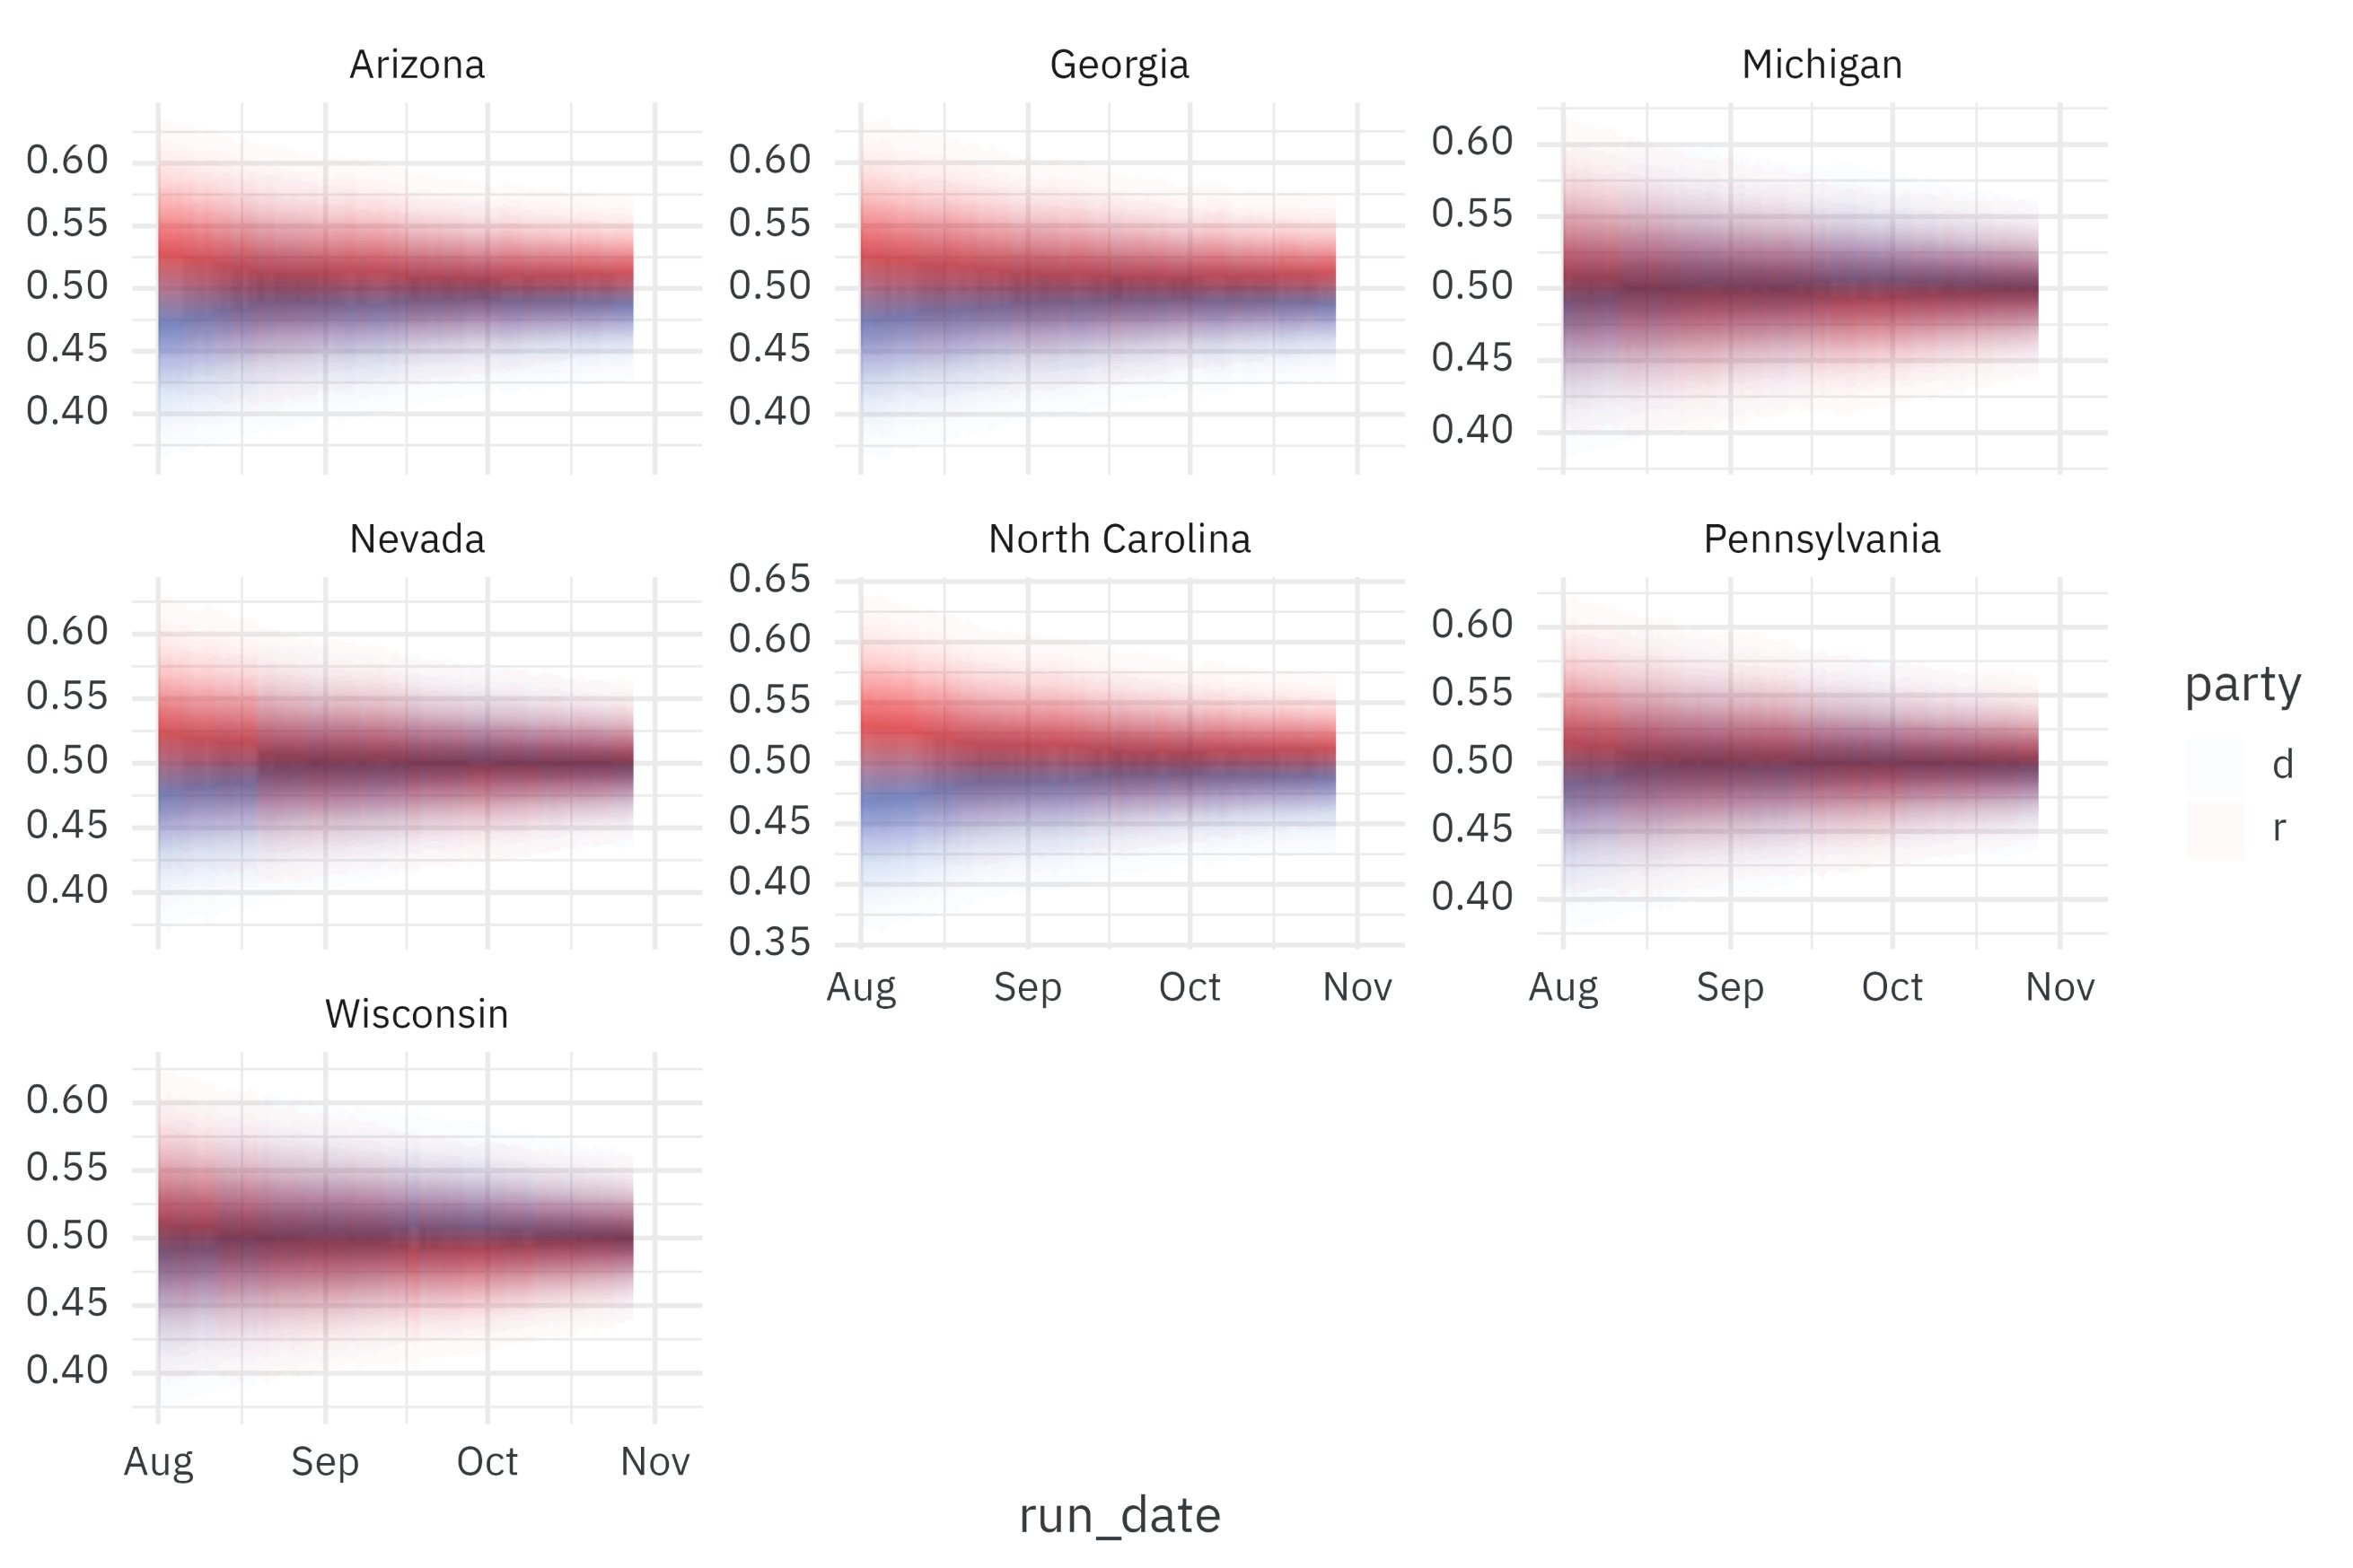
\includegraphics[height = .8\textheight]{mark_rieke_uncertainty.jpeg}
}
}

\end{document}
